\documentclass[conference]{IEEEtran}
\IEEEoverridecommandlockouts

\usepackage{cite}
\usepackage{amsmath,amssymb}
\usepackage{graphicx}
\usepackage{booktabs}
\usepackage{url}
\usepackage[hidelinks,pdfauthor={},pdfcreator={},pdfproducer={}]{hyperref}
\hypersetup{pdftitle={Leak-Safe Probabilistic Demand Forecasting on M5: Kalman, LightGBM, a Kalman-LightGBM Hybrid and DeepAR}}

% Figures are reused from the evidence package; nothing is copied.
\graphicspath{{../docs/figures/eda/}}

\newcommand{\WAPE}{\mathrm{WAPE}}
\newcommand{\avail}{a}

\begin{document}

\title{Leak-Safe Probabilistic Demand Forecasting on M5:\\
Kalman Filtering, LightGBM, a Kalman--LightGBM Hybrid and DeepAR}

\author{\IEEEauthorblockN{Anonymous Submission}
\IEEEauthorblockA{Phase~1 (Machine Learning) project report}}

\maketitle

\begin{abstract}
Inventory decisions need demand quantiles rather than single point forecasts, and retail sales are sparse, zero-heavy counts that are partly censored by stockouts. We compare a per-series Kalman filter, a direct multi-horizon LightGBM model, a hybrid that feeds Kalman state estimates to LightGBM, the DeepAR global network and an equal-weight quantile ensemble. All models run under one rolling-origin protocol in which each model receives only history up to the forecast origin. The data are a frozen subset of the M5 competition: 1,200 series from three Walmart stores over 1,000 days. Over four 28-day test origins (124,992 evaluated cells on established series), DeepAR has the lowest weighted absolute percentage error (WAPE 0.697 against 0.772 for a four-week seasonal naive benchmark). On mean pinball loss DeepAR (0.26191), the hybrid (0.26198) and the ensemble (0.26231) are tied within the variation across origins. The hybrid is best on days not flagged as stockouts (WAPE 0.660, pinball 0.269) and has the lowest WAPE on simulated cold-start series (0.760). The Kalman filter equals a 28-day moving average in accuracy but runs about 29 times faster than LightGBM. DeepAR's 90\% intervals over-cover (0.965). Ablations show that a negative binomial likelihood outperforms a Gaussian one for DeepAR, and that masking proxy-flagged stockout days improves accuracy on non-flagged days. Stockout flags are a heuristic proxy because M5 contains no inventory records. Hyperparameters were not tuned and each model was run with a single seed.
\end{abstract}

\begin{IEEEkeywords}
demand forecasting, intermittent demand, Kalman filter, LightGBM, DeepAR, quantile forecasting, M5, stockout censoring
\end{IEEEkeywords}

%======================================================================
\section{Introduction}
%======================================================================
A replenishment decision is a bet on a range of future demand. In the newsvendor model, the cost-minimising order level is the $q^{*}=C_u/(C_u+C_o)$ quantile of demand, where $C_u$ is the unit cost of a lost sale and $C_o$ the unit cost of holding excess stock. If a lost sale costs nine times as much as holding a unit, $q^{*}=0.9$. A forecaster that reports only a mean leaves the planner to guess the spread, so we evaluate full sets of quantiles with proper scoring rules~\cite{gneiting2007}.

Daily retail sales make this harder. In our M5 subset, 59\% of the days on which items are offered for sale record zero sales, and 90\% of series are classified as intermittent or lumpy (Section~\ref{sec:data}). Some zero runs are probably stockouts rather than absent demand. M5 provides no inventory data, so such censoring can only be inferred.

This report addresses one question: \emph{under a single leak-safe protocol, how do a local state-space model, a tabular gradient-boosting model, a hybrid of the two, and a global deep model compare on accuracy, calibration and cost for sparse retail demand?} Its contributions are:
\begin{enumerate}
\item a rolling-origin benchmark on a frozen 1,200-series M5 subset, in which every model receives a context that is truncated at the forecast origin;
\item a stockout-proxy rule, applied identically to all models, that masks suspected censored days and never imputes them;
\item results on established series, on days not flagged as stockouts, and on simulated cold-start series, together with the ablations that were completed. Experiments that were not run are listed explicitly.
\end{enumerate}

%======================================================================
\section{Related Work}
%======================================================================
\textbf{Intermittent demand.} Croston's method smooths nonzero demand sizes and inter-demand intervals separately~\cite{croston1972}. Syntetos and Boylan showed that it is biased and proposed a correction (SBA)~\cite{syntetos2005accuracy}. TSB updates a demand probability every period so that forecasts decay for obsolescent items~\cite{teunter2011}. These methods give point forecasts and use no covariates or seasonality. The ADI/CV$^2$ classification of Syntetos, Boylan and Croston~\cite{syntetos2005categorization} divides series into smooth, erratic, intermittent and lumpy. We use it to report results by demand class. Snyder, Ord and Beaumont~\cite{snyder2012} model intermittent demand with count distributions.

\textbf{Classical statistical models.} Exponential smoothing in state-space form~\cite{hyndman2002} and automatic ARIMA~\cite{hyndman2008} are standard per-series methods with Gaussian errors. They are weak on sparse counts and use few covariates. Croston, SBA, TSB, ETS and ARIMA are cited here for context only; \emph{none of them is implemented as a baseline in this study}.

\textbf{State-space models and the Kalman filter.} The Kalman filter~\cite{kalman1960} gives recursive estimates of a hidden state. Structural time-series models express a level and seasonal pattern as such states~\cite{harvey1989,durbin2012}. Missing observations are handled by skipping the update step, which lets us mask censored days without imputing them.

\textbf{Tree-based and global models.} LightGBM~\cite{ke2017} is a fast gradient-boosted tree library. Trained on lag, calendar and price features, it was widely used among the leading M5 accuracy entries~\cite{makridakis2022accuracy}. A \emph{global} model fits one set of parameters across many series. Global models can borrow strength from related series and can produce forecasts for series with little history~\cite{januschowski2020,montero2021}. DeepAR~\cite{salinas2020} is a global autoregressive recurrent network with a parametric output likelihood. It produces probabilistic forecasts by sampling paths.

\textbf{Benchmarks and evaluation.} The M5 competitions~\cite{makridakis2022accuracy,makridakis2022uncertainty} found that simple seasonal benchmarks are hard to beat, and that combining forecasts and using cross-series learning usually help. Pinball loss is a proper scoring rule for quantiles~\cite{gneiting2007}. Kolassa~\cite{kolassa2016} discusses why evaluating count forecasts needs care. Hyndman and Koehler~\cite{hyndman2006} review the problems of percentage-based error measures on low-volume data. These problems motivate the aggregated WAPE used here.

\textbf{Gap.} The individual methods are all established. To our knowledge, few studies compare a local state-space model, a tabular GBDT and a global deep model under one leak-safe rolling-origin protocol that also treats censoring and calibration consistently across every model. We present our contribution as a careful comparison, not as a new method.

%======================================================================
\section{Data, Quality and Exploratory Analysis}\label{sec:data}
%======================================================================
\subsection{Subset and data contract}
We use \texttt{sales\_train\_evaluation.csv}, \texttt{calendar.csv} and \texttt{sell\_prices.csv} from M5. The subset contains 400 items from each of the stores CA\_1, TX\_1 and WI\_1, chosen by stratified sampling with seed 42 and frozen in \texttt{configs/subsets/m5\_subset.csv}. It covers the last 1,000 days, from 2013-08-27 to 2016-05-22. By category the series are FOODS 566, HOUSEHOLD 410 and HOBBIES 224. An adapter converts the files into a target matrix $Y\in\mathbb{R}_{\ge0}^{N\times T}$, an availability mask $\avail\in\{0,1\}^{N\times T}$, known-future covariates $K\in\mathbb{R}^{N\times T\times 23}$ and static attributes. A day counts as available if its week has a posted sell price, and 95.64\% of cells are available.

\subsection{Quality checks}
The raw subset has no duplicate series identifiers, no negative sales and no missing cells. The 701,313 weekly price rows contain no duplicate store--item--week keys and no missing or non-positive prices. The processed grid has no NaN targets on available cells. Every exploratory statistic in this section is computed over the full 1,000-day window, including the test period. These statistics are descriptive only and are \emph{not} given to any model. Inside the backtest, masks and demand classes are recomputed from data available before the relevant cutoff (Section~\ref{sec:leak}).

\subsection{Sparsity and demand classes}
Fig.~\ref{fig:zero} shows that, after early launches settle, about 60\% of available series sell nothing on a given day. Across all launched and available cells the zero share is 59.11\%, and mean demand is 1.25 units per series-day. For the classification we compute ADI as available days divided by the number of nonzero sales, and CV$^2$ as the squared coefficient of variation of the nonzero sale sizes. With the cut-offs 1.32 and 0.49 (Fig.~\ref{fig:adi}), the 1,200 series split into 914 intermittent, 167 lumpy, 89 smooth and 30 erratic. The backtest computes these classes before the first origin and for established series only, which gives different counts: 839 intermittent, 162 lumpy, 87 smooth, 27 erratic and 1 new item among 1,116 series. Mean demand varies across series by orders of magnitude (Appendix Fig.~\ref{fig:cv}). This spread motivates count likelihoods and per-series scaling.

\begin{figure}[t]
\centering
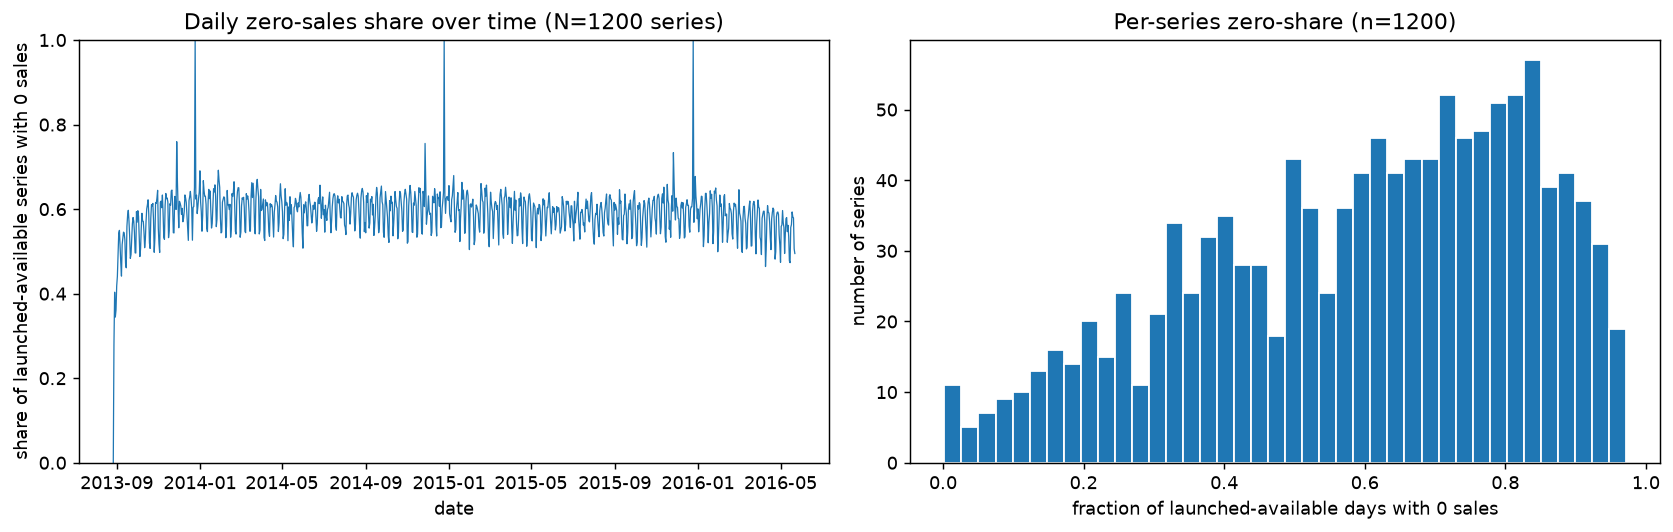
\includegraphics[width=\columnwidth]{01_zero_share.png}
\caption{Left: daily share of launched, available series with zero sales. Right: per-series zero share. The low values at the start reflect series not yet launched, not a demand pattern.}
\label{fig:zero}
\end{figure}

\begin{figure}[t]
\centering
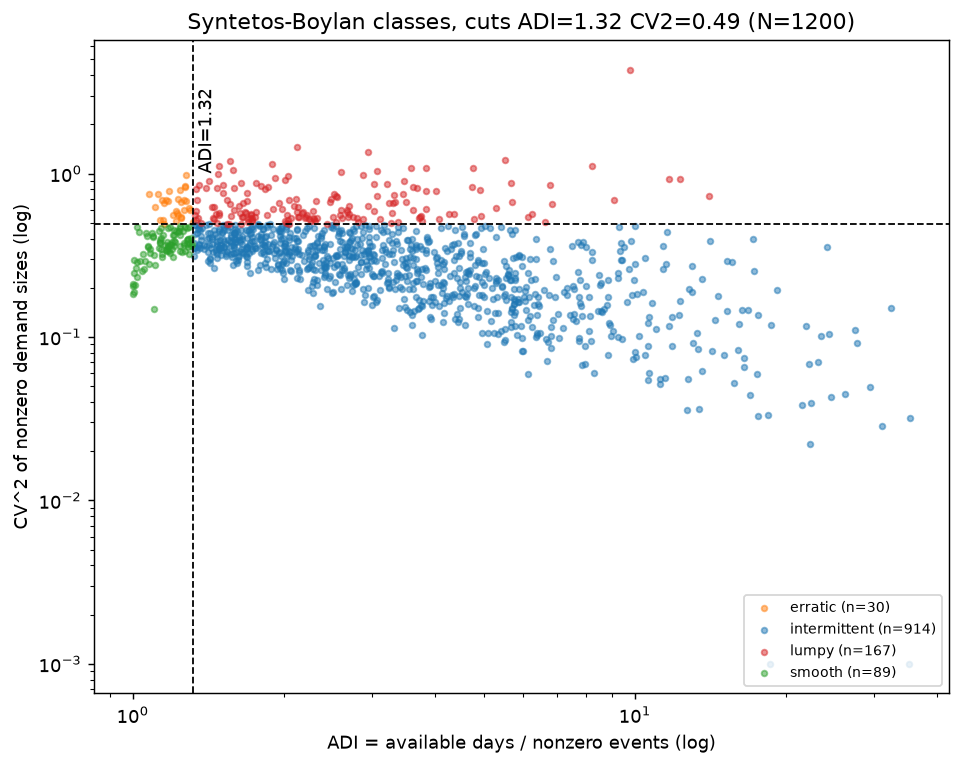
\includegraphics[width=0.92\columnwidth]{02_adi_cv2.png}
\caption{Syntetos--Boylan classification of the 1,200 series over the full window. Dashed lines mark ADI $=1.32$ and CV$^2=0.49$.}
\label{fig:adi}
\end{figure}

\subsection{Calendar, SNAP and price patterns}
The clearest seasonal signal is the day of the week (Fig.~\ref{fig:season}). Mean sales on Saturdays and Sundays are 1.26 to 1.31 times the category mean. The monthly profile varies much less. Mean sales on event days are 0.934 times those on non-event days. SNAP benefits are paid on state-specific days, so we compare SNAP and non-SNAP days within each state. Mean sales on SNAP days are 1.070 (CA), 1.107 (TX) and 1.058 (WI) times those on non-SNAP days. All of these are descriptive associations, not causal effects. In 56.75\% of series the price changes at least once, and the median absolute weekly change is 8.2\%. Within a series, weeks priced below the series mean have higher mean relative sales (Appendix Fig.~\ref{fig:price}). This pattern motivates the price covariates, but it does not identify price elasticity.

\begin{figure}[t]
\centering
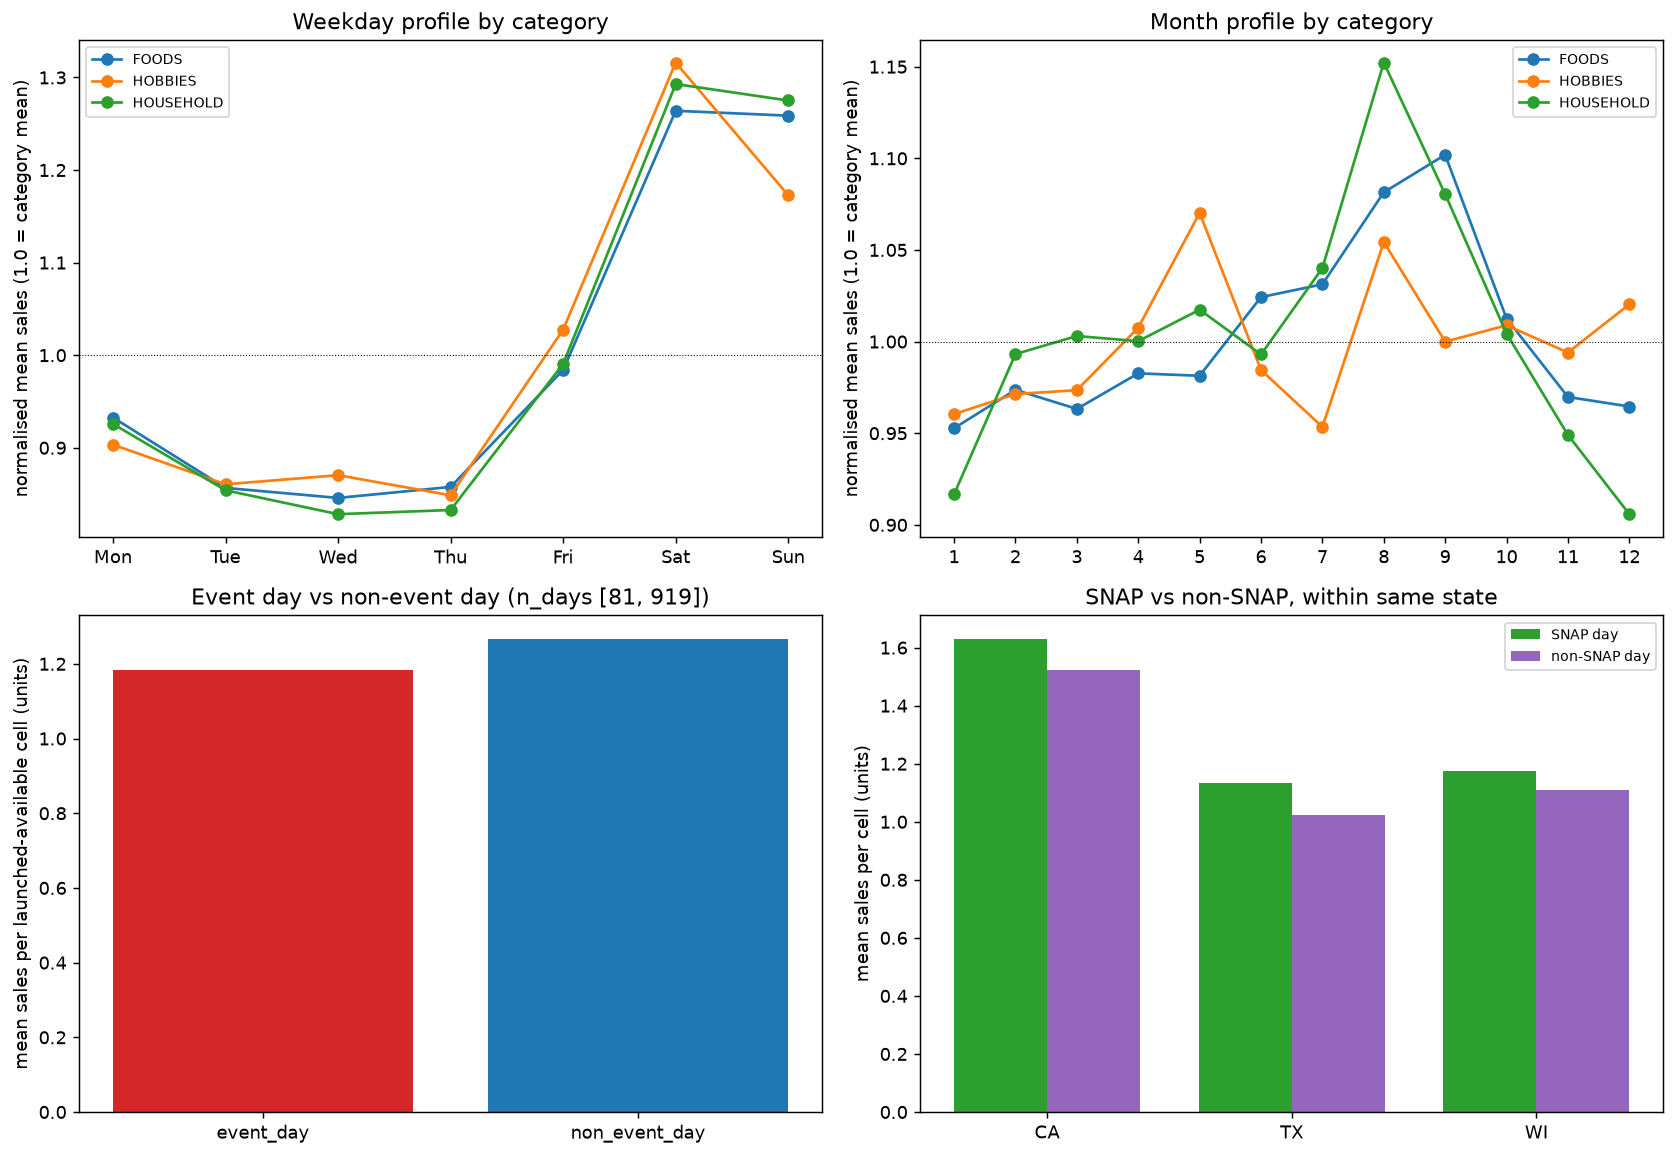
\includegraphics[width=\columnwidth]{04_seasonality_event_snap.png}
\caption{Normalised mean sales by weekday and by month for each category, with event-day and within-state SNAP comparisons. All comparisons are descriptive.}
\label{fig:season}
\end{figure}

\subsection{Stockout proxy}\label{sec:proxy}
For a series with at least $n_{\min}=10$ nonzero sales, a run of available zero days of length $L$ is flagged if
\begin{equation}
L \ge \max\!\left(L_{\min},\; \kappa\cdot\mathrm{ADI}\right),\qquad L_{\min}=28,\ \kappa=3.
\label{eq:proxy}
\end{equation}
In words, a zero run is flagged only when it is much longer than the series' usual gap between sales, and only for series that sell regularly. Over the full window the rule flags 12.97\% of cells in 1,948 runs (Fig.~\ref{fig:stockout}). In the benchmark, where the rule is applied to established-series test cells, 8.69\% of cells are flagged. The rule is a heuristic, not a measurement. It produces false positives for genuine quiet periods and seasonal items. It produces false negatives for short outages, partial stockouts and items with fewer than 10 sales. A flagged zero is never treated as confirmed lost demand.

\begin{figure}[t]
\centering
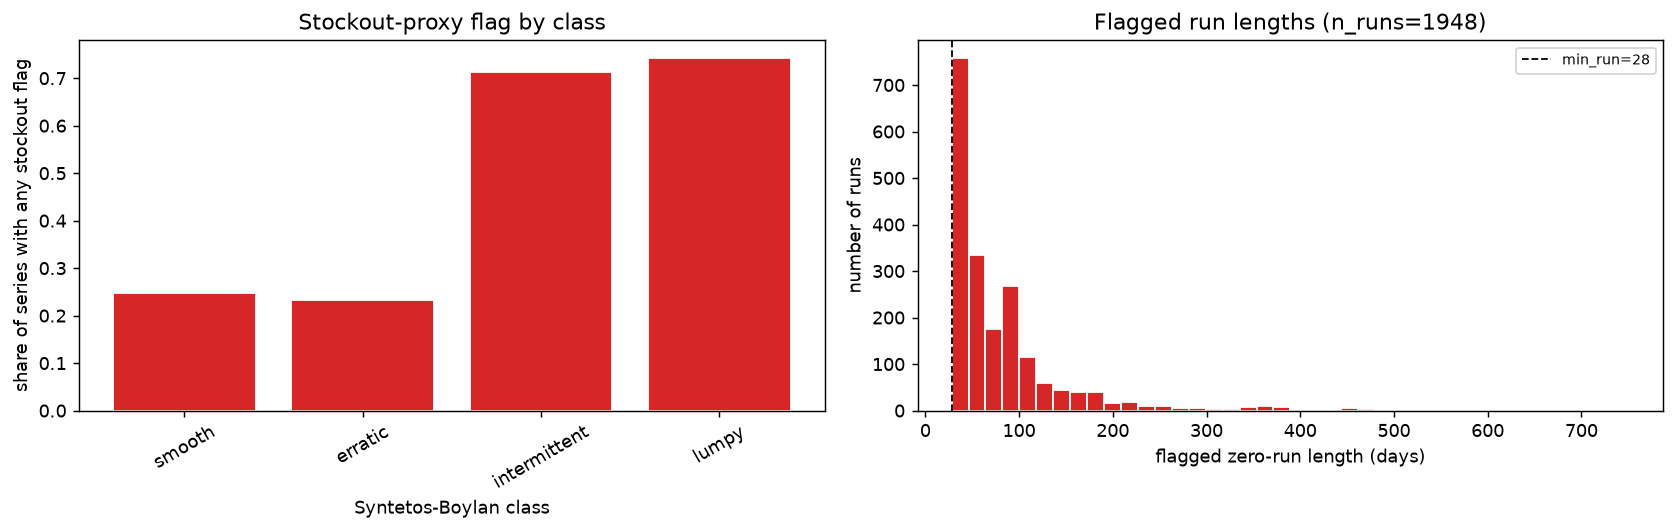
\includegraphics[width=\columnwidth]{06_stockout.png}
\caption{Stockout-proxy flags over the full window. Left: share of series with at least one flagged run, by demand class. Right: lengths of flagged zero runs. These flags are rule outputs, not observed stockouts.}
\label{fig:stockout}
\end{figure}

%======================================================================
\section{Feature Engineering and Leakage Prevention}\label{sec:features}
%======================================================================
\subsection{Features}
The LightGBM model uses 59 features, listed in Table~\ref{tab:feat}. Lag, rolling and recency features are computed at an \emph{anchor} day $t$ from targets up to $t$. Known-future covariates are read at the target day $t+h$. The four rolling statistics are computed over windows of 7, 14, 28, 56 and 112 days, and each skips masked days: the mean, the standard deviation, the share of days with nonzero sales, and the masked fraction. The weekday-aligned lags $\text{slag}_k$ take the value on the same weekday as the target day, from the most recent week at or before $t$ and the three weeks before it. \texttt{item\_id} is \emph{not} a LightGBM feature in the main run (\texttt{use\_item\_id=false}). The hybrid adds three Kalman features: the filtered level, the one-step predictive standard deviation, and the $h$-step state-space mean $Z T^{h} a_t$.

\begin{table}[t]
\caption{LightGBM feature groups (59 features; the hybrid adds 3)}
\label{tab:feat}
\centering
\footnotesize
\begin{tabular}{@{}p{0.56\columnwidth}rp{0.27\columnwidth}@{}}
\toprule
Group & $n$ & Read at \\
\midrule
Horizon $h$ & 1 & -- \\
Target lags $y_t, y_{t-1}, y_{t-2}$ & 3 & anchor $t$ \\
Weekday lags $\text{slag}_{1..4}$, their mean & 5 & $\le t$ \\
Rolling mean, std, nonzero rate, mask fraction & 20 & window to $t$ \\
Days since sale, age, mean to date & 3 & anchor $t$ \\
Calendar (13), events (5), SNAP (1) & 19 & target day $t{+}h$ \\
Price: log price, weekly change, ratio to 26-week past mean, promo flag & 4 & target day $t{+}h$ \\
Static: dept, category, store, state & 4 & -- \\
\midrule
Hybrid only: $\hat\ell_{t|t}$, $\mathrm{sd}_1$, $ZT^{h}a_t$ & 3 & anchor $t$ \\
\bottomrule
\end{tabular}
\end{table}

\textbf{Price assumption.} The price features are read at the target week. This follows the M5 convention that sell prices are published in advance. The price-change and past-mean features use only earlier weeks. \texttt{log\_price}, however, uses the posted price of the target week, so it is leak-free \emph{only} if prices really are known ahead. On datasets where they are not, these features should be lagged to the origin. In weeks with no posted price, \texttt{log\_price} is filled with the series' mean log price over the whole window. These cells are unavailable and never scored, but this fill value is not strictly causal.

\textbf{Feature importance.} We do not report feature importance. The main run did not save the trained LightGBM boosters, and computing gain importance would require retraining, which was outside the scope of Phase~1. Gain importance would in any case indicate association, not causation.

\subsection{Leakage controls}\label{sec:leak}
At an origin $T_0$, the forecasting context contains only $Y_{:,0:T_0}$. Future targets are not present in the object passed to a model. Leading-zero and stockout masks are recomputed on this history slice. The demand classes used for slice reporting are computed before the first test origin. LightGBM training rows satisfy $t+h\le T_0$. A unit test replaces every target after the origin with random integers and checks three things: the context arrays are unchanged; the quantiles and means of six model families (seasonal naive, moving average, Kalman, LightGBM, hybrid, DeepAR) agree to within $10^{-5}$; and the tabular features and stockout flags are unchanged. This test checks one specific kind of perturbation on a small fixture. It is strong evidence against \emph{target} leakage but does not prove that no leak exists. In particular, it cannot detect a covariate built with future information inside the adapter, such as the price fill described above.

%======================================================================
\section{Models}\label{sec:models}
%======================================================================
\subsection{Baselines}
The baselines are the naive forecast (last value), the seasonal naive forecast (the same weekday one week earlier, \textsf{snaive}), the average of the same weekday over the last four weeks (\textsf{snaive4}, which is the reference model), and a 28-day moving average (\textsf{ma28}).

\subsection{Kalman filter (local)}
Each series is modelled on the scale $z_t=\sqrt{y_t}$ with a local level $\ell_t$ and a stochastic weekly seasonal term $\gamma_t$ ($m=7$):
\begin{align}
z_t &= \ell_t + \gamma_t + \varepsilon_t, & \varepsilon_t&\sim\mathcal N(0,\sigma^2),\\
\ell_{t+1} &= \ell_t + \xi_t, & \xi_t&\sim\mathcal N(0,q_\ell\sigma^2),\\
\gamma_{t+1} &= -\textstyle\sum_{j=0}^{m-2}\gamma_{t-j} + \omega_t, & \omega_t&\sim\mathcal N(0,q_s\sigma^2).
\end{align}
The state is $\alpha_t=(\ell_t,\gamma_t,\dots,\gamma_{t-5})^\top$ with observation vector $Z=(1,1,0,\dots,0)$. The predicted state is $a_{t|t-1}$ with covariance $P_{t|t-1}$. The innovation is $v_t=z_t-Za_{t|t-1}$ and its variance is $F_t=ZP_{t|t-1}Z^\top+1$. On a day where $y_t$ is missing, unavailable or flagged by the stockout proxy, the update step is skipped and the state is only propagated. The scale $\sigma^2$ is concentrated out of the likelihood: $\hat\sigma^2=\tfrac1n\sum v_t^2/F_t$, giving $\log L=-\tfrac12\,(n\log\hat\sigma^2+\sum\log F_t)$, with the first 14 observations excluded as burn-in. In the main run $(q_\ell,q_s)$ is chosen \emph{per series by grid search} over $q_\ell\in\{10^{-3},10^{-2},3\cdot10^{-2},10^{-1}\}$ and $q_s\in\{0,10^{-4},10^{-3},10^{-2}\}$, maximising $\log L$ on the last 365 days. Series with fewer than 28 observations use the fixed pair $(10^{-2},10^{-3})$. No EM algorithm is used. The filter starts from a diffuse prior $P_0=10^{3}I$. Quantiles are computed as $g^{-1}(\mu_h+\Phi^{-1}(p)\sqrt{V_h})$ and clipped at zero, where $\mu_h$ and $V_h$ are the $h$-step predictive mean and variance and $g^{-1}(x)=x^2$.

\subsection{LightGBM (direct multi-horizon)}
The 28 horizons are split into four buckets: days 1--7, 8--14, 15--21 and 22--28. Each bucket has one Poisson model for the mean and one LightGBM quantile model per level $q\in\{0.05,0.1,0.25,0.5,0.75,0.9,0.95\}$, so 32 boosters are trained per origin with 200 trees each. The learning rate is 0.06, with 63 leaves, a minimum of 80 samples per leaf, feature and bagging fractions of 0.8, and an L2 penalty of 1. Training rows come from anchors spaced 7 days apart over the last 364 days, and rows whose target is masked are dropped. Because the horizon $h$ is itself a feature, a bucket model can still tell its horizons apart. This direct design does not feed predictions back as inputs, so one-step errors do not compound. The costs are more models, less data per horizon, and no joint coherence across horizons. Quantiles from all models are clipped at zero and sorted, which removes quantile crossing.

\subsection{Kalman--LightGBM hybrid}
The hybrid is LightGBM plus the three Kalman features in Table~\ref{tab:feat}. They come from a filter run on the last 514 days (\texttt{train\_days}+150) with one noise-ratio pair shared across all series, which is the default setting of the hybrid. The idea is that the local filter supplies an adaptive level and an uncertainty estimate for each series, while the global booster learns how to combine them with covariates across series. The hybrid uses classical and ML components only; it contains no deep-learning part.

\subsection{DeepAR (global)}
DeepAR is a 2-layer LSTM with 64 hidden units and dropout 0.1, shared across all series. At each step $t$ its input is the previous target divided by the scale $\nu=1+\bar y_{\text{context}}$, an indicator of whether that target was observed, $\log\nu$, the 23 covariates, and learned embeddings of the item (8 dimensions) and of the department, category, store and state (4 dimensions each). Its output parameterises a negative binomial distribution with mean $\mu_t=\nu\,\mathrm{softplus}(w_\mu^\top h_t)$ and dispersion $\alpha_t=\mathrm{softplus}(w_\alpha^\top h_t)/\sqrt{\nu}$. The negative log-likelihood is averaged only over available, non-masked targets. Training uses windows with an 84-day context and Adam (learning rate $10^{-3}$, weight decay $10^{-5}$, cosine schedule, gradient clipping at 10). The first origin is trained for 2,500 steps, and each later origin is fine-tuned for 800 steps starting from the previous weights. During training the item embedding is replaced by an ``unknown'' index with probability 0.15, and cold-start series always use this index. Quantiles are computed from 200 sampled paths.

\subsection{Ensemble}
The ensemble averages the quantiles of the Kalman filter, LightGBM and DeepAR with equal weights of 1/3. It is applied after forecasting and involves no extra training.

%======================================================================
\section{Experimental Setup and Metrics}\label{sec:setup}
%======================================================================
\textbf{Rolling origins.} There are four test origins, 2016-01-31, 2016-02-28, 2016-03-27 and 2016-04-24, spaced 28 days apart, each with horizon $H=28$ (the M5 horizon). The last test window ends on 2016-05-22. One earlier validation origin (2016-01-03) is reserved for tuning, but \emph{tuning was not run}. All models use the hand-set configuration in \texttt{configs/m5.yaml}.

\textbf{Evaluation sets.} A cell is one (origin, series, horizon) combination. We evaluate three sets:
\begin{itemize}
\item \emph{All days}: the 1,116 established series over all available days, giving $1{,}116\times28\times4=124{,}992$ cells.
\item \emph{Non-censored}: the same cells minus those flagged by the proxy, giving 114,127 cells.
\item \emph{Simulated cold start}: 84 series (7\%) for which only the last 28 days of history are visible and global models receive the unknown-item embedding, giving 9,408 cells.
\end{itemize}
These cold-start series are existing products with history hidden. They are not genuinely new products. For the flags used in scoring, the base rule is applied to the full series and kept fixed across ablation variants, so every variant is scored on the same cells.

\textbf{Metrics.} Let $\mathcal V$ be the set of valid cells, $y$ the actual value, $\hat y^{(0.5)}$ the median forecast and $\bar y$ the mean forecast. Then
\begin{gather}
\mathrm{MAE}=\tfrac{1}{|\mathcal V|}\textstyle\sum_{\mathcal V}|y-\hat y^{(0.5)}|,\quad
\WAPE=\dfrac{\sum_{\mathcal V}|y-\hat y^{(0.5)}|}{\sum_{\mathcal V}y},\\
\mathrm{RMSE}=\Big(\tfrac{1}{|\mathcal V|}\textstyle\sum_{\mathcal V}(y-\bar y)^2\Big)^{1/2}.
\end{gather}
WAPE is a ratio of sums over all cells, not an average of per-series ratios. For a quantile level $q$ with error $u=y-\hat y^{(q)}$, the pinball loss is $\rho_q(u)=\max(qu,(q-1)u)$. The reported \emph{pinball} is $\rho_q$ averaged over the seven quantile levels and over $\mathcal V$, without scaling. The weighted quantile loss is $\mathrm{WQL}=\tfrac{1}{|Q|}\sum_q 2\sum_{\mathcal V}\rho_q/\sum_{\mathcal V}y$. Cov80 and Cov90 are the shares of actuals inside $[\hat y^{(0.1)},\hat y^{(0.9)}]$ and $[\hat y^{(0.05)},\hat y^{(0.95)}]$, with inclusive bounds. Inclusive bounds are generous for zero-heavy counts. Significance against \textsf{snaive4} is tested with a paired bootstrap over series: 1,000 resamples, recomputing each aggregate metric, with a 95\% percentile interval.

%======================================================================
\section{Results}\label{sec:results}
%======================================================================
\subsection{Main comparison}
Table~\ref{tab:main} gives the all-days results. DeepAR has the lowest WAPE (0.697) and MAE (0.891), a 9.7\% lower WAPE than \textsf{snaive4}. The top three pinball scores are DeepAR 0.26191, the hybrid 0.26198 and the ensemble 0.26231. The gaps between them are at most 0.0004, while each model's pinball loss has a standard deviation of about 0.004 across origins. We therefore treat these three as tied on pinball loss and do not claim a probabilistic winner. The hybrid improves on plain LightGBM on every point and quantile metric in the table, though by small margins (WAPE 0.704 against 0.709). The ensemble has the lowest RMSE (1.782), and its Cov90 of 0.919 is closer to nominal than that of LightGBM, the hybrid or DeepAR. It is not the best model overall. DeepAR's intervals are too wide: Cov80 is 0.931 and Cov90 is 0.965.

The Kalman filter matches \textsf{ma28} (WAPE 0.7226 against 0.7222). It takes 13.7\,s across all four origins, about 29 times faster than LightGBM (397\,s) and 22 times faster than DeepAR (296\,s), measured on an 8-core Apple M3 CPU. In the paired bootstrap, every learned model beats \textsf{snaive4} on both WAPE and pinball, with confidence intervals that exclude zero. For example, DeepAR's WAPE difference is $-0.076$ $[-0.086,-0.067]$ and the hybrid's pinball difference is $-0.028$ $[-0.031,-0.024]$. These tests compare each model only with \textsf{snaive4}. They do not test the top models against each other.

\begin{table*}[t]
\caption{Established series, all days, four origins (124,992 cells). Lower is better except coverage (nominal 0.80/0.90). Time: fit plus predict over all origins.}
\label{tab:main}
\centering
\begin{tabular}{@{}lcccccccr@{}}
\toprule
Model & MAE & RMSE & WAPE & Pinball & WQL & Cov80 & Cov90 & Time (s)\\
\midrule
Naive & 1.413 & 2.733 & 1.104 & 0.4244 & 0.664 & 0.822 & 0.892 & 0.1\\
Seasonal naive (1 wk) & 1.148 & 2.296 & 0.898 & 0.3375 & 0.528 & 0.880 & 0.933 & 0.1\\
Seasonal naive (4 wk), reference & 0.988 & 1.901 & 0.772 & 0.2899 & 0.453 & 0.838 & 0.914 & 0.2\\
Moving average (28 d) & 0.924 & 1.864 & 0.722 & 0.2744 & 0.429 & 0.811 & 0.891 & 0.2\\
Kalman (local) & 0.924 & 1.917 & 0.723 & 0.2736 & 0.428 & 0.831 & 0.914 & 13.7\\
LightGBM & 0.907 & 1.799 & 0.709 & 0.26366 & 0.412 & 0.871 & 0.941 & 397.4\\
Kalman--LightGBM hybrid & 0.900 & 1.798 & 0.704 & 0.26198 & 0.410 & 0.875 & 0.940 & 441.0\\
DeepAR & \textbf{0.891} & 1.790 & \textbf{0.697} & 0.26191 & \textbf{0.409} & 0.931 & 0.965 & 295.5\\
Ensemble (Kalman, LightGBM, DeepAR) & 0.899 & \textbf{1.782} & 0.703 & 0.26231 & 0.410 & 0.827 & 0.919 & --\\
\bottomrule
\end{tabular}
\end{table*}

\subsection{Non-censored days and cold start}
On non-censored days (Table~\ref{tab:slices}) the hybrid is best on both WAPE (0.65981) and pinball loss (0.26928), ahead of LightGBM (0.66295 / 0.27071) and DeepAR (0.66480 / 0.27226). DeepAR therefore ranks first on WAPE when flagged days are included and third when they are excluded. The masking ablation in Section~\ref{sec:abl} explains this reversal. On simulated cold start the hybrid has the lowest WAPE (0.760), MAE and RMSE. LightGBM and DeepAR both reach a WAPE of 0.773, and LightGBM has the lowest cold-start pinball loss (0.27359). The plain Kalman filter does worst among the learned models on cold start (WAPE 0.839), and its diffuse prior produces wide intervals.

\begin{table}[t]
\caption{Non-censored days (114,127 cells) and simulated cold start (9,408 cells)}
\label{tab:slices}
\centering
\small
\begin{tabular}{@{}lcccc@{}}
\toprule
& \multicolumn{2}{c}{Non-censored} & \multicolumn{2}{c}{Cold start}\\
\cmidrule(lr){2-3}\cmidrule(l){4-5}
Model & WAPE & Pinball & WAPE & Pinball\\
\midrule
\textsf{snaive4} & 0.759 & 0.309 & 0.875 & 0.319\\
\textsf{ma28} & 0.712 & 0.293 & 0.783 & 0.292\\
Kalman & 0.686 & 0.282 & 0.839 & 0.323\\
LightGBM & 0.663 & 0.2707 & 0.773 & \textbf{0.2736}\\
Hybrid & \textbf{0.660} & \textbf{0.2693} & \textbf{0.760} & 0.2748\\
DeepAR & 0.665 & 0.2723 & 0.773 & 0.2775\\
Ensemble & 0.665 & 0.2706 & 0.783 & 0.283\\
\bottomrule
\end{tabular}
\end{table}

\subsection{By demand class and volume}
The ranking also depends on the slice. On the 93,968 intermittent cells, DeepAR has the lowest WAPE (0.810, against 0.827 for the hybrid). On erratic series (0.722) and on low-volume series (1.007) the hybrid is best. On smooth series all learned models are close (WAPE 0.454 to 0.463). The new-item slice contains one series and is not interpreted.

\subsection{Ablations}\label{sec:abl}
Only the variants listed in Table~\ref{tab:abl} were run. For each, the all-days and non-censored metrics are shown.

\begin{table}[t]
\caption{Completed ablations (all days / non-censored)}
\label{tab:abl}
\centering
\footnotesize
\begin{tabular}{@{}lcccc@{}}
\toprule
Variant & WAPE & Pinball & WAPE$_{nc}$ & Pinball$_{nc}$\\
\midrule
\multicolumn{5}{@{}l}{\emph{Kalman (base: sqrt, per-series grid, 365 d, masked)}}\\
base & 0.723 & 0.2736 & 0.686 & 0.2822\\
shared ratio & \textbf{0.718} & \textbf{0.2686} & \textbf{0.680} & \textbf{0.2772}\\
fixed ratio & 0.725 & 0.2736 & 0.688 & 0.2816\\
log1p transform & 0.744 & 0.2860 & 0.701 & 0.2900\\
no transform & 0.786 & 0.2792 & 0.731 & 0.2857\\
window 180 d & 0.728 & 0.2777 & 0.693 & 0.2868\\
no masking & 0.701 & 0.2698 & 0.694 & 0.2907\\
\midrule
\multicolumn{5}{@{}l}{\emph{DeepAR (base: negative binomial, masked; main run)}}\\
base & 0.697 & 0.2619 & 0.665 & \textbf{0.2723}\\
no loss masking & \textbf{0.677} & \textbf{0.2565} & 0.669 & 0.2760\\
Gaussian likelihood & 0.792 & 0.2784 & 0.732 & 0.2853\\
\bottomrule
\end{tabular}
\end{table}

\textbf{Masking.} Removing the stockout mask improves the all-days scores for both models but worsens the non-censored scores (Kalman pinball 0.2907 against 0.2822; DeepAR 0.2760 against 0.2723). DeepAR's cold-start pinball loss is also worse without masking (0.293 against 0.278). The scoring flags are the same for every variant. The all-days set contains the flagged zero days, and an unmasked model learns to predict exactly those zeros, so it scores better on them. Its non-censored score is worse. If the proxy flags really are mostly stockouts, the non-censored set is the closer estimate of accuracy on true demand, and masking helps there. This conclusion depends on how accurate the proxy is.

\textbf{Likelihood.} Replacing the negative binomial with a Gaussian raises DeepAR's WAPE from 0.697 to 0.792 (a 12.1\% increase) and its pinball loss from 0.2619 to 0.2784 (5.9\%). It also worsens cold-start WAPE (0.888 against 0.773). The negative binomial matches nonnegative, overdispersed counts, while the Gaussian puts probability on negative values.

\textbf{Kalman design.} The square-root transform matters: with no transform WAPE rises to 0.786. With the log1p transform, the mean back-transform $\exp(\mu+V/2)-1$ amplifies large states and RMSE rises to 20.6. A single noise-ratio pair shared across all series slightly beats the per-series grid on every column, which suggests that the per-series search overfits on this subset. A 180-day estimation window is worse than 365 days. The DeepAR base row is taken from the main run with the same configuration and seed. It was not re-run inside the ablation.

%======================================================================
\section{Discussion, Limitations and Threats to Validity}
%======================================================================
\textbf{Interpretation.} DeepAR is the most accurate model under the all-days aggregate point metrics. The hybrid is best when flagged days are excluded and on simulated cold start. On pinball loss the leading models are tied. The hybrid's gain over LightGBM is consistent across the reported views but small. Kalman features are switched on or off together, so we cannot say which feature produces the gain. The Kalman filter offers no accuracy gain over \textsf{ma28}, but it is cheap and its state can be interpreted. As the hybrid shows, its value here is mainly as an input to a global model.

\textbf{Calibration.} With inclusive bounds, coverage is generous for zero-heavy counts. If a lower quantile and the actual are both zero, the actual counts as covered. For each quantile level the evaluator therefore reports two shares, $P(y\le\hat y^{(q)})$ and $P(y<\hat y^{(q)})$. For a calibrated forecast of discrete data, $q$ lies between them, within a tolerance of 0.02. DeepAR falls inside this band at all seven levels, LightGBM and the hybrid at six (all except 0.75), the Kalman filter at six (all except 0.5), and the ensemble at four (0.05, 0.1, 0.9, 0.95). DeepAR's Cov90 of 0.965 is above nominal under the inclusive-bound definition, and part of this excess comes from ties at zero. We do not claim that any model is calibrated overall.

\textbf{Threats to validity.}
\begin{itemize}
\item \emph{Proxy labels.} Stockout flags come from Eq.~\eqref{eq:proxy}, not from inventory data. They affect both training and the non-censored evaluation set.
\item \emph{Scope.} The data are one retailer, three stores and 1,200 series, with four origins all in early 2016 and a single seed (42). We report no variation across seeds.
\item \emph{No tuning.} The hyperparameters are hand-set and identical across origins. Tuned baselines could change the ranking among closely matched models.
\item \emph{Simulated cold start.} Hiding history from existing products does not reproduce real product launches.
\item \emph{Covariate assumptions.} The price features assume prices are known in advance, and the price gap fill is not strictly causal (Section~\ref{sec:features}).
\item \emph{Missing baselines.} Croston, SBA, TSB, ETS and ARIMA were not run, so the comparison does not cover these intermittent and classical methods.
\end{itemize}

%======================================================================
\section{Conclusion and Future Work}
%======================================================================
Under one leak-safe rolling-origin protocol on 1,200 M5 series, every learned model significantly beats a four-week seasonal naive benchmark. DeepAR gives the lowest all-days WAPE. DeepAR, the Kalman--LightGBM hybrid and the equal-weight ensemble are tied on pinball loss. The hybrid leads on non-censored days and on simulated cold start. Two findings from the completed ablations are supported: a count likelihood clearly improves DeepAR, and stockout masking helps on non-flagged days.

The following experiments are defined in the repository but were \emph{not} run:
\begin{itemize}
\item the LightGBM ablation (Tweedie and L2 objectives, no price features, 14-day buckets, item ID, no masking);
\item the stockout-rule ablation (a 14-day minimum run, and no masking for all models);
\item the remaining DeepAR variants (no item ID, no price covariates, 56- and 112-day contexts);
\item hyperparameter tuning on the validation origin, evaluation over multiple seeds, and LightGBM feature importance;
\item the intermittent-demand baselines Croston, SBA and TSB.
\end{itemize}
Recalibrating DeepAR's quantiles on the validation origin is a further direction.

\section*{Reproducibility}
All numbers come from \texttt{outputs/m5\_main/report/} (\texttt{forecastkit all configs/m5.yaml}) and from the Kalman and DeepAR ablation directories. The figures are produced by \texttt{scripts/eda\_m5.py}. The test suite has 35 tests and all pass.

\bibliographystyle{IEEEtran}
\bibliography{references}

\appendix
\section*{Supplementary EDA figures}

\begin{figure}[h]
\centering
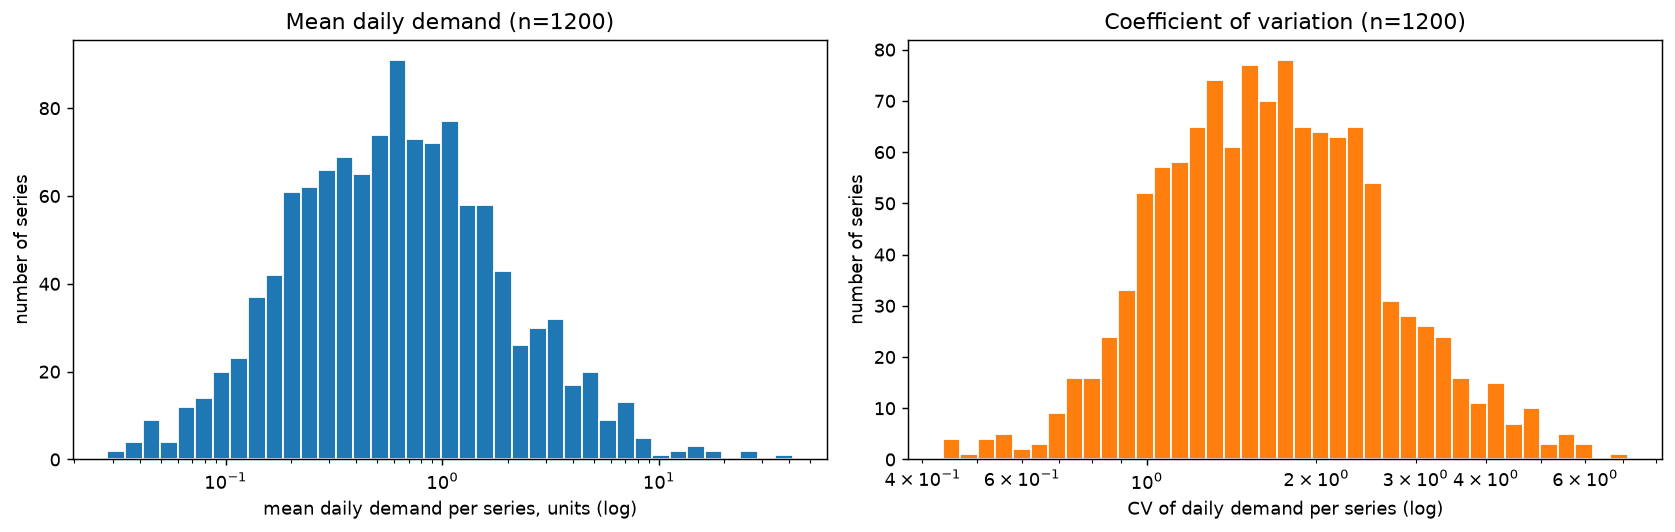
\includegraphics[width=\columnwidth]{03_demand_cv.png}
\caption{Distribution across series of mean daily demand and of the coefficient of variation (log scale). The CV includes zero days, so it is high for sparse series by construction.}
\label{fig:cv}
\end{figure}

\begin{figure}[h]
\centering
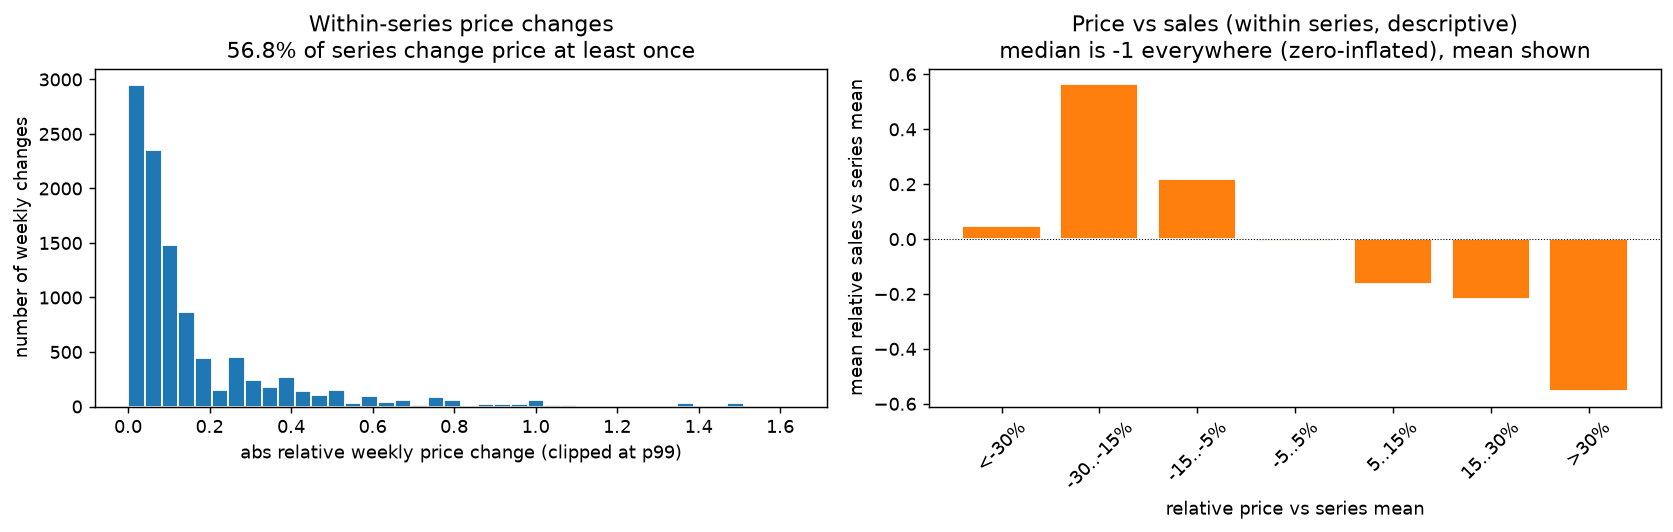
\includegraphics[width=\columnwidth]{05_price.png}
\caption{Left: absolute weekly relative price changes. Right: mean relative sales within series, by price relative to the series mean. The plot shows means because the median is $-1$ in every bin (most days are zero). The relationship is descriptive, not causal.}
\label{fig:price}
\end{figure}

\end{document}
